% !TEX root = ../CedricDe Schepper2023_Thesis.tex

\section{Threats to Validity}\label{sec:threats}

In this section, we discuss the threats to the validity of the analyses performed. The presence of these threats could undermine the trustworthiness of the obtained results, and negatively impact the quality of this thesis. For every threat, we look at how we were able to mitigate it.


% Figure~\ref{fig:threats} shows a diagram of the experiment principles and where lies each threat.
% Please do not use this image on the paper/thesis.
% Reviewers are supposed to know where the threats lie, the figure is for students to better understand the threats.
% \begin{figure}[H]
% 	\centering
% 	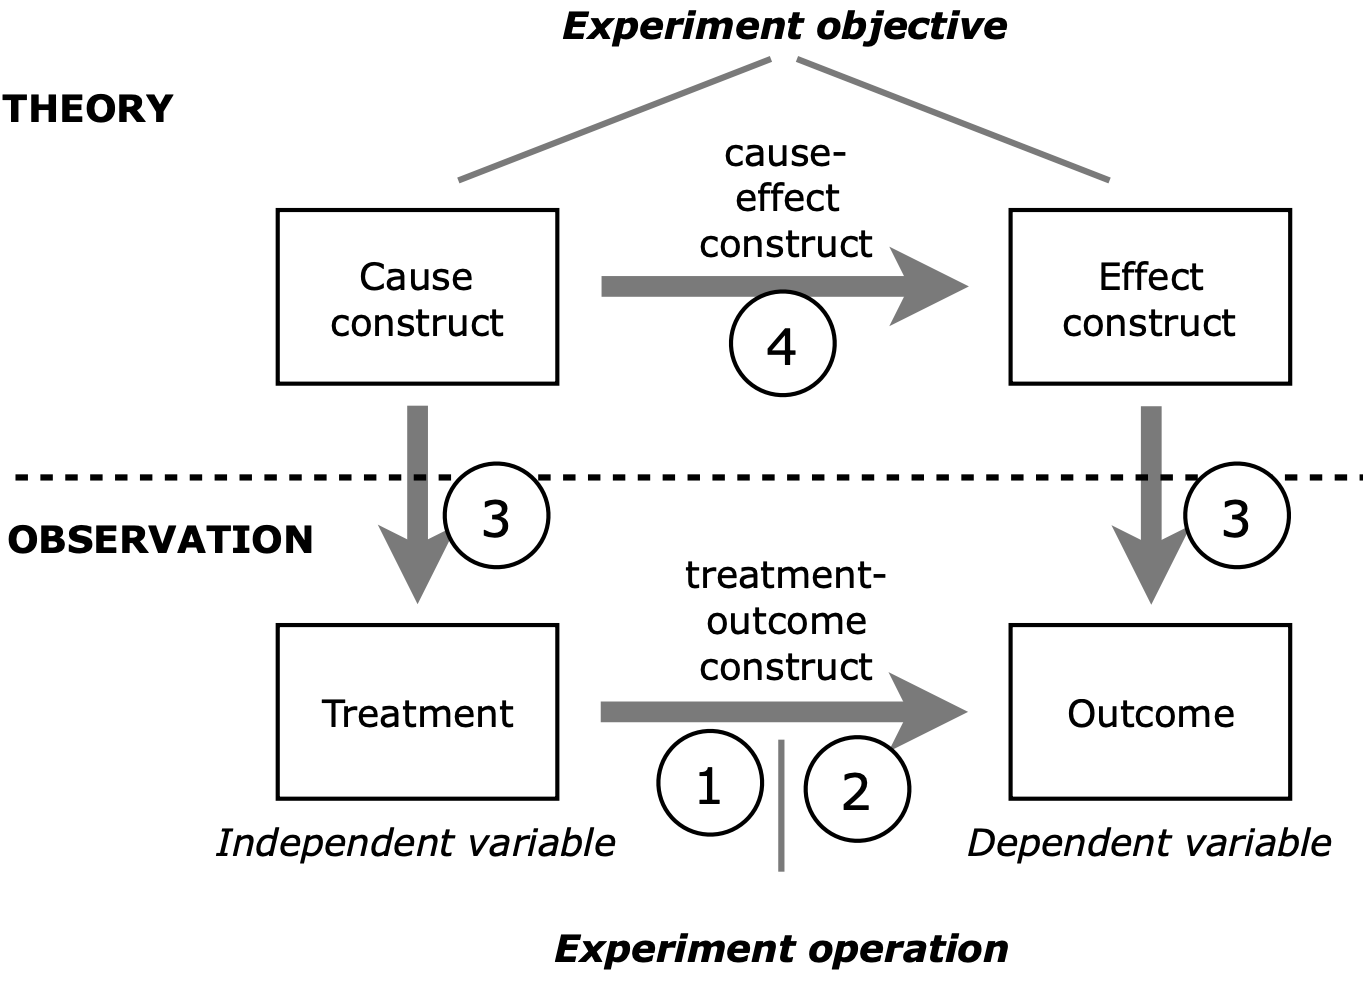
\includegraphics[width=0.75\textwidth]{images/threats-to-validity.png} 
% 	\caption{Experimental principles diagram showing threats. (1) Conclusion; (2) Internal; (3) Construct; and (4) External.}
% 	\label{fig:threats}
% \end{figure}


\subsection{Conclusion validity}

Conclusion validity refers to the reliability of the conclusions drawn from the generated results. Since only two data sets were used during the analyses, this could pose a threat to the validity of those results. However, the characteristics and size of the data set help in mitigating this threat. Both data sets consist of data from two faculties, and add up to a notable size. The size and workload statistics of the provided data sets were compared with several instances for the Toronto benchmark in Table \ref{tab:workload_compared}, discussed in Section \ref{sec:experiment}. This showed that the sizes of the data sets provided are competitive compared to the Toronto benchmark, especially when taking the workload into account.


% Conclusion validity is the degree to which conclusions we reach about relationships in our data are reasonable.
% \begin{itemize}
%    \item  It affects the ability to draw correct conclusion about relations between treatment and outcome. \\
% + Choice of statistical tests \\
% + Choice of sample size \\
% + Measurement of the experiment
%   \item Low Statistical Power \\
% + If power is low, there is a high risk that an erroneous conclusion is drawn.
% \end{itemize}

\subsection{Internal validity}

Threats to the internal validity of analyses risk impacting the trustworthiness of the results observed. These threats were mitigated in several ways. First, the randomness in generating the initial solution helps preventing bias from infiltrating the results. Additionally, all analyses were run multiple times in order to verify that the results obtained were robust and to remove outliers. Overall, it was observed that all the results produced  were similar.


% Are there any other factors that may affect the results?
% \begin{itemize}
%   \item Were phenomena observed under special conditions \\
% + in the lab, close to a deadline, company risked bankruptcy, … \\
% + major turnover in team, contributors changed (open-source), …
%   \item Similar observations repeated over time (learning effects)
%   \item Correlation does not imply causation.
% \end{itemize}

\subsection{Construct validity}

The construct validity threat focuses on how accurately the scoring metrics assess the quality of solutions. The objective function and exam distribution are the two main scoring metrics used. The objective function is based on the objective function by Alvarez-Valdes et al. \cite{alvarez1997}. Additionally, the use of the exam distribution metric has been discussed and accepted as a valid metric by the University's administration in order to rate the quality of solutions.

\subsection{External validity}

The external validity threat refers to the generalisability of the findings, namely to what extend the findings can be applied to other situations. The use case presented by data and constraints of the University of Antwerp timetabling problem did not fit within any of the existing benchmarks. This could create a potential threat to the external validity of our analyses. However, the improvements applied to the original algorithm are generic in nature. For example, Version 3, as detailed in Section \ref{version3}, expands the amount of search space explored during every iteration. This expansion does not take into account any specificities of our use case and can be applied to all timetabling problems.

% A possible threat to the external validity of our experiments can be the 
% To what extent can the findings be generalized?
% \begin{itemize}
%   \item Does it apply to other languages? Other sizes? Other domains? Other systems?
%   \item Background \& education of participants
%   \item Simplicity \& scale of the team \\
% + small teams \& flexible roles vs. large organizations \& fixed roles
% \end{itemize}